\section{Конструкторский раздел}

\subsection{Схемы алгоритмов}

На рисунке \ref{scheme-main} представлен основной алгоритм работы родительского процесса сервера.

\begin{figure}[H]
	\centering
	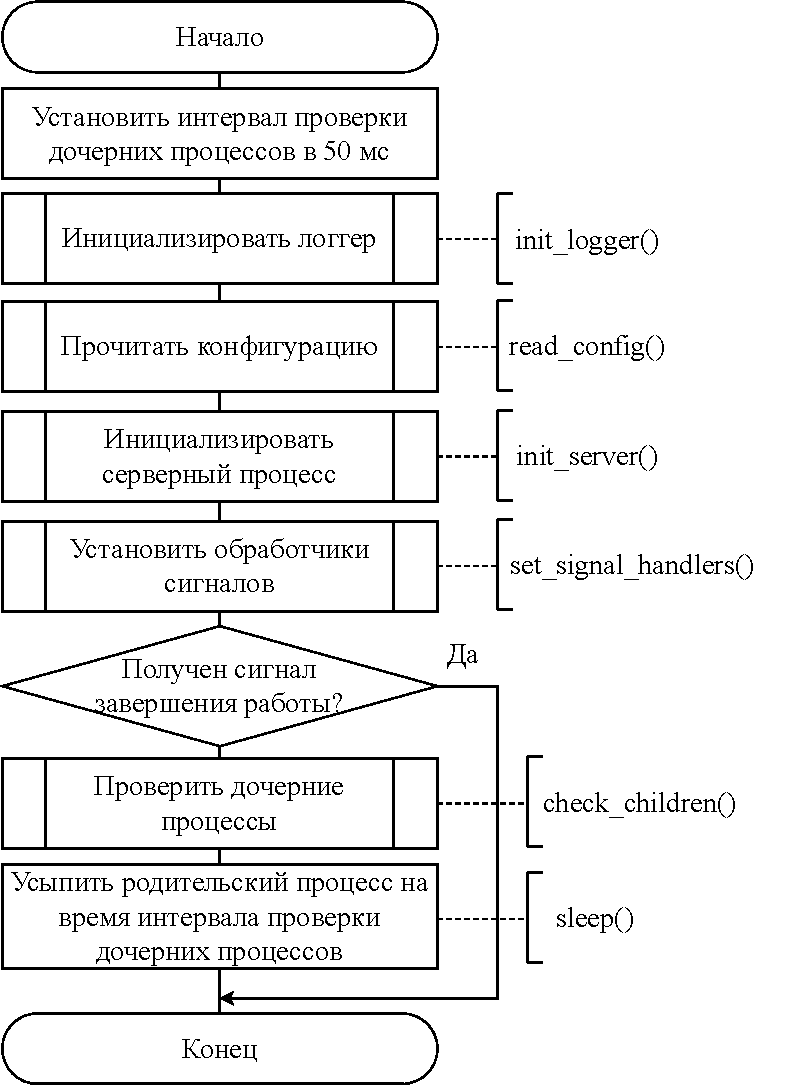
\includegraphics[scale=0.9]{img/main.pdf}
	\caption{Алгоритм работы процесса-родителя}
	\label{scheme-main}
\end{figure}

\newpage

На рисунке \ref{scheme-init-server} представлен алгоритм функции инициализации сервера.

\begin{figure}[H]
	\centering
	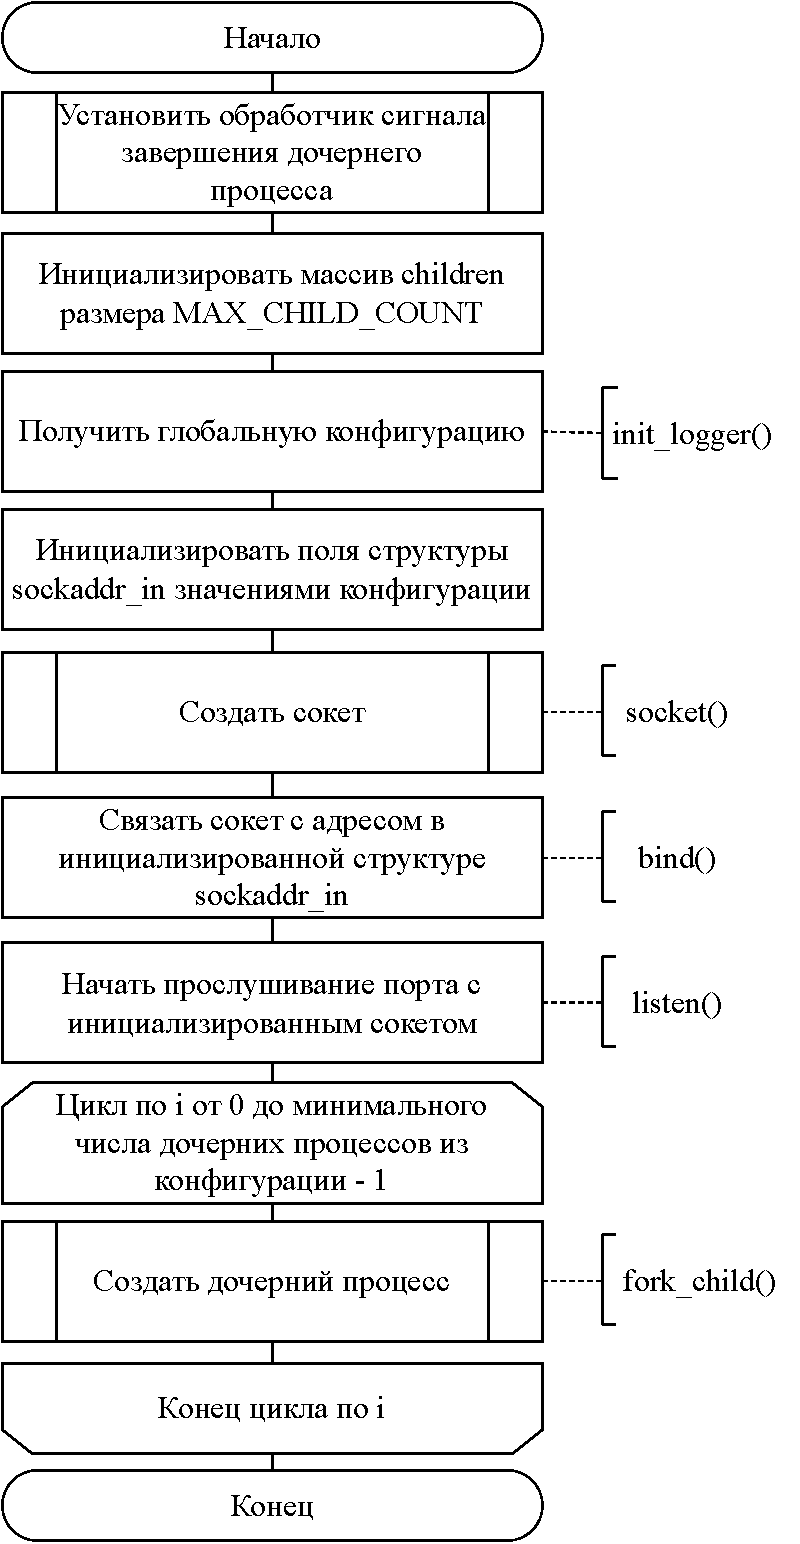
\includegraphics[scale=0.8]{img/init_server.pdf}
	\caption{Алгоритм функции init\_server()}
	\label{scheme-init-server}
\end{figure}

\newpage

На рисунке \ref{scheme-fork-child} представлен алгоритм создания дочернего процесса сервера.

\begin{figure}[H]
	\centering
	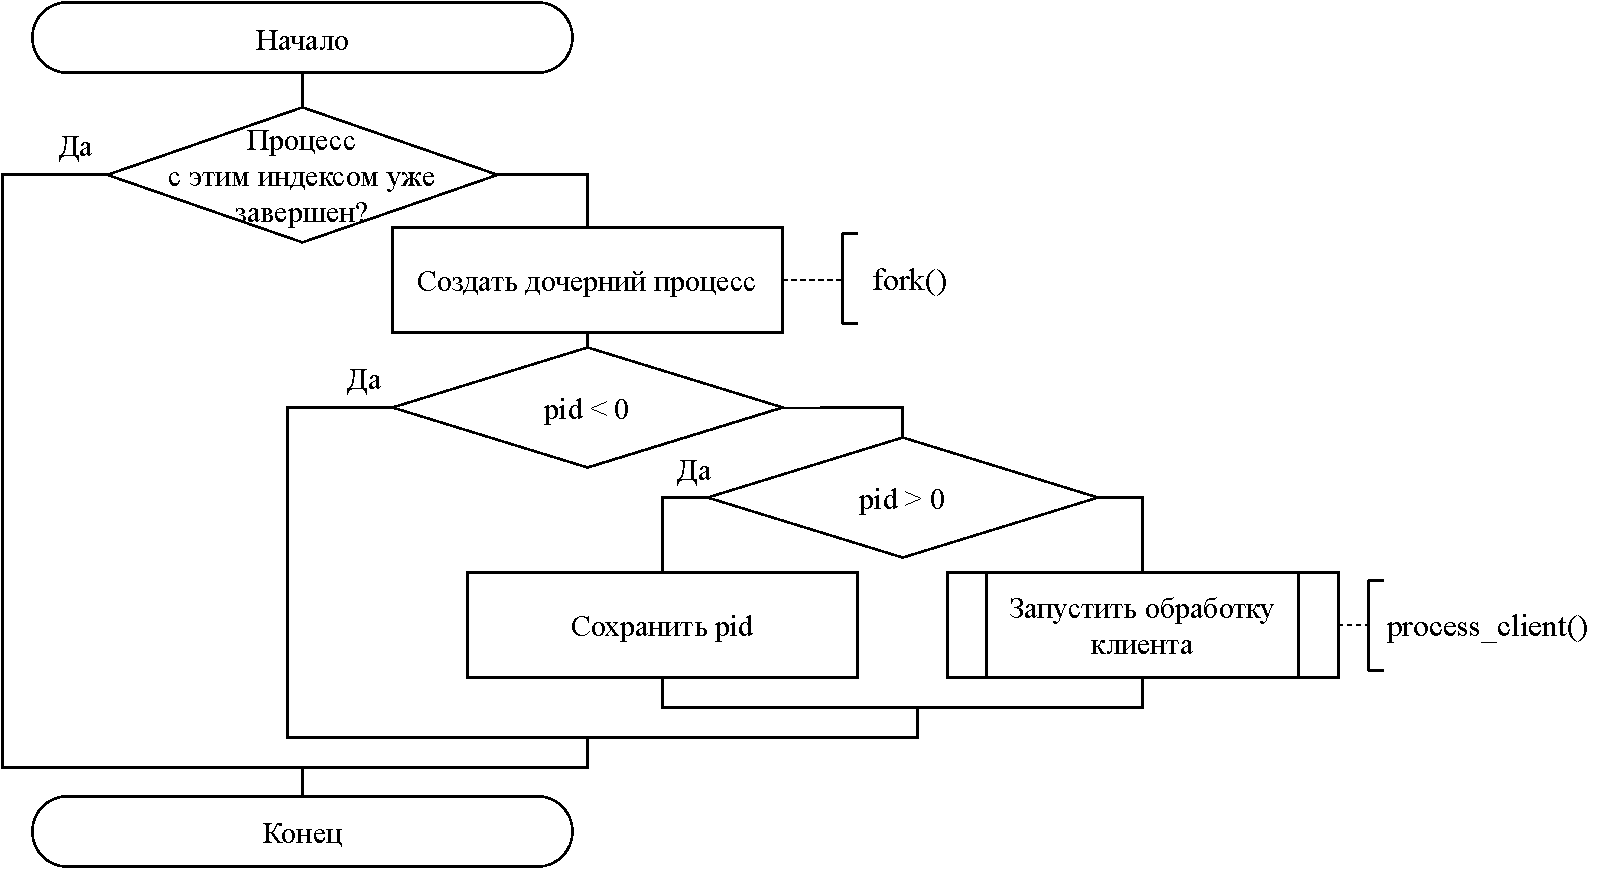
\includegraphics[scale=0.6]{img/fork_child.pdf}
	\caption{Алгоритм функции fork\_child()}
	\label{scheme-fork-child}
\end{figure}

На рисунке \ref{scheme-process-client} представлен алгоритм функции инициализации дочернего процесса.

\begin{figure}[H]
	\centering
	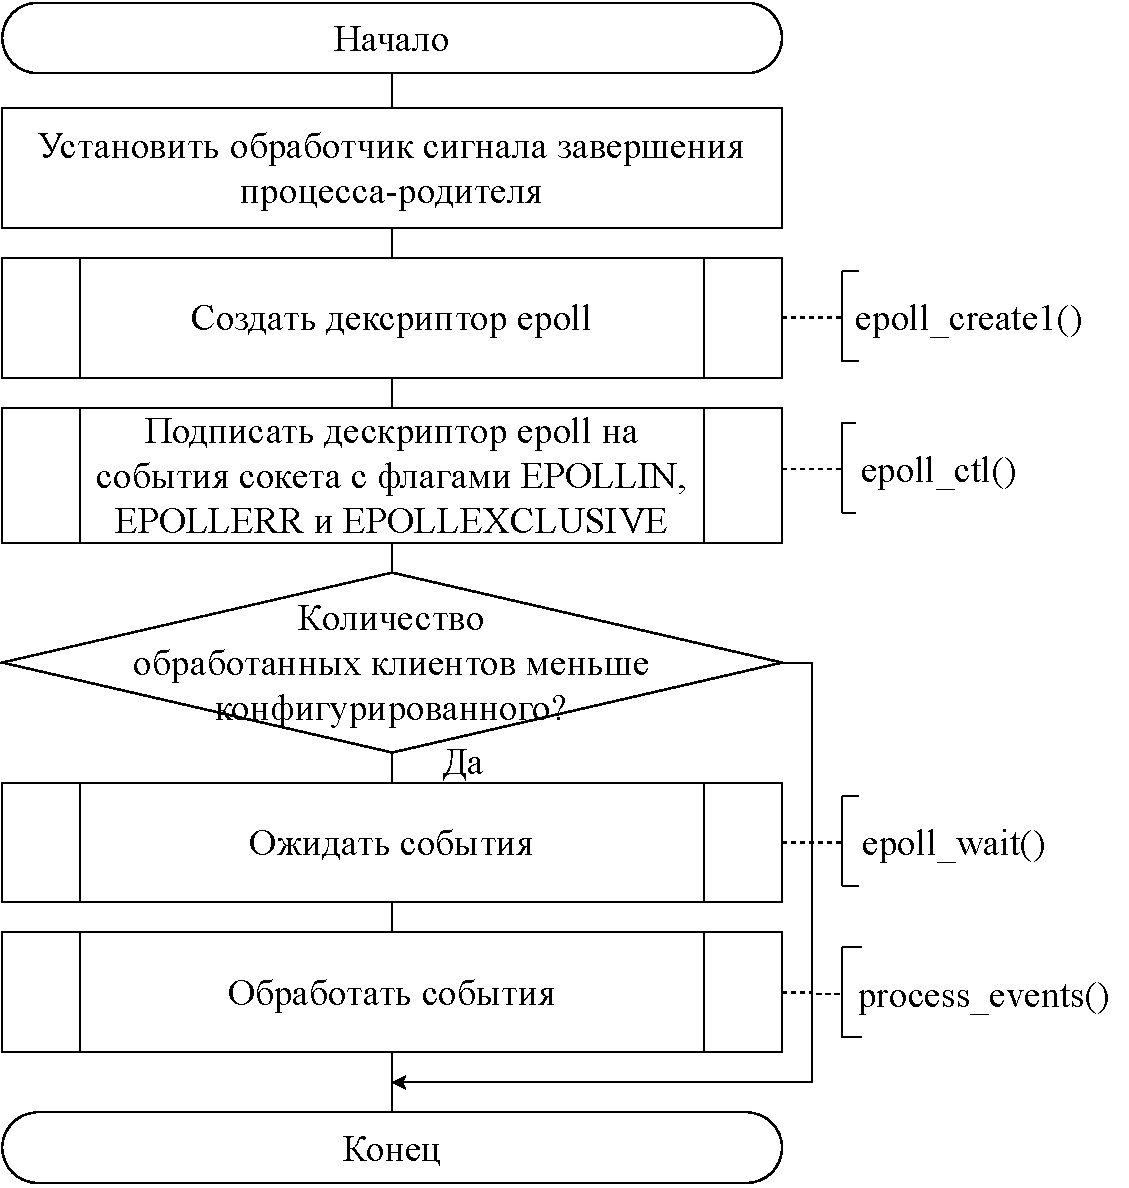
\includegraphics[scale=0.5]{img/process_client.pdf}
	\caption{Алгоритм функции process\_client()}
	\label{scheme-process-client}
\end{figure}

На рисунке \ref{scheme-process-events} представлен алгоритм функции обработки события в виде запроса.

\begin{figure}[H]
	\centering
	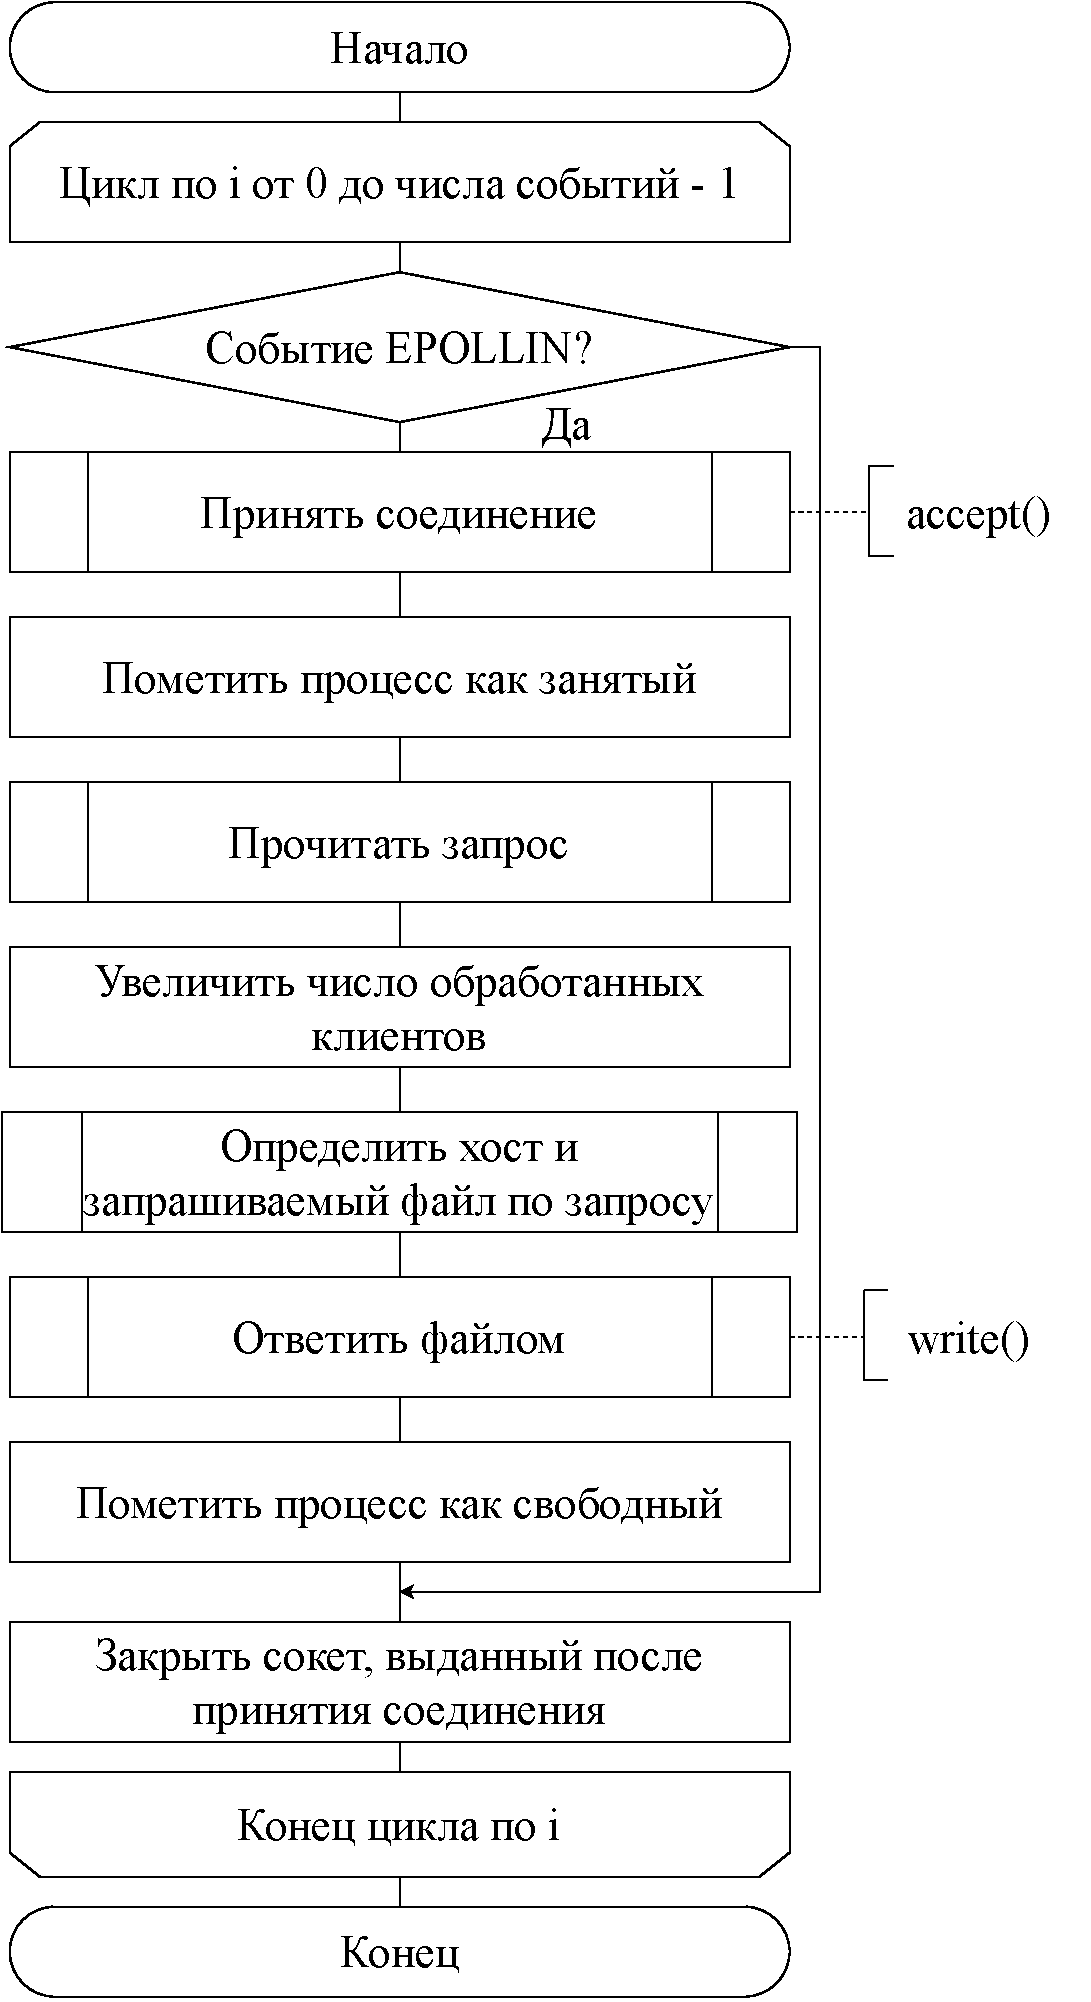
\includegraphics[scale=0.6]{img/process_events.pdf}
	\caption{Алгоритм функции process\_events()}
	\label{scheme-process-events}
\end{figure}

\newpage

На рисунке \ref{scheme-check-children} представлен алгоритм функции регулярной проверки пула процессов.

\begin{figure}[H]
	\centering
	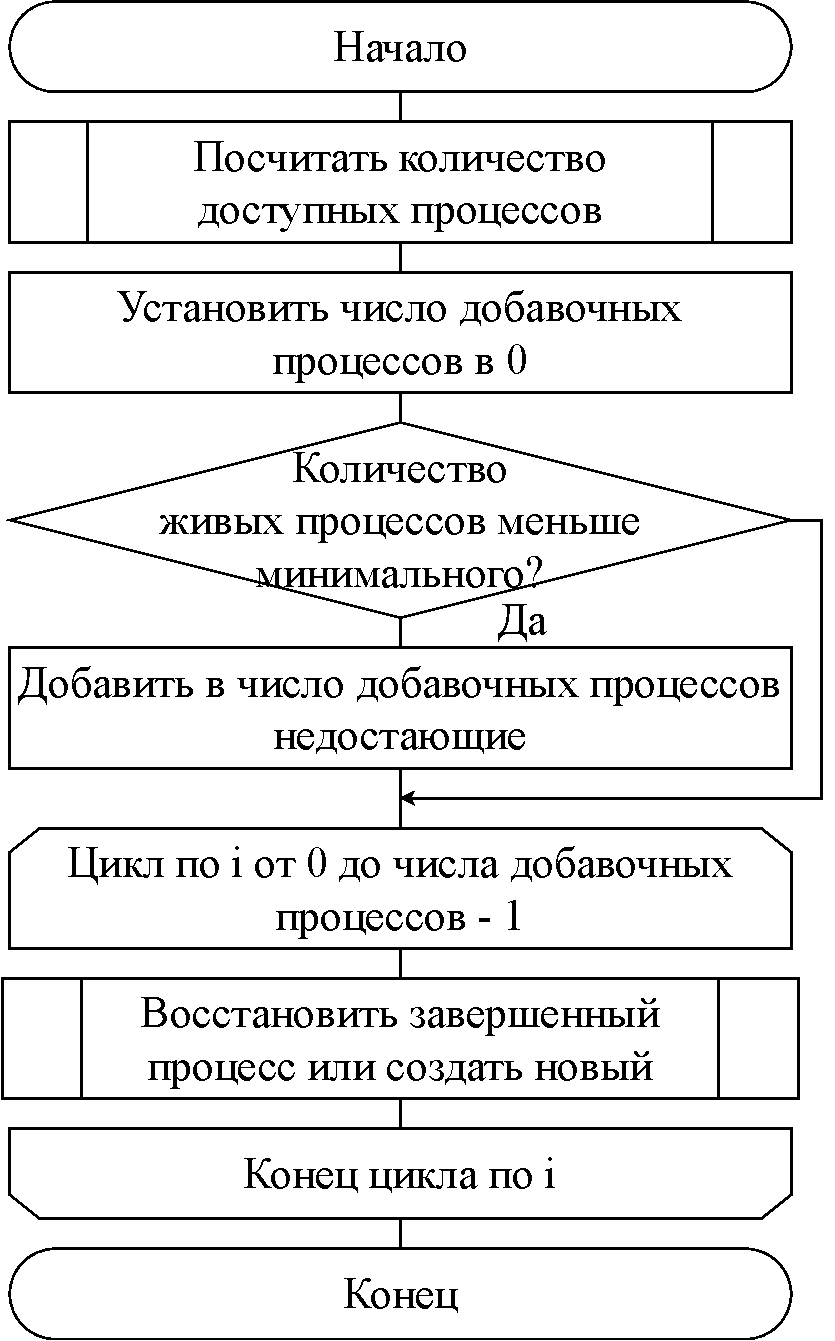
\includegraphics[scale=0.6]{img/check_children.pdf}
	\caption{Алгоритм функции check\_children()}
	\label{scheme-check-children}
\end{figure}

\subsection{Проектирование компонентов системы}

Для решения поставленной задачи спроектировано следующее разделение системы на программные компоненты:

\begin{enumerate}
	\item config -- модуль для работы с конфигурацией,
	
	\item http -- набор модулей для работы с заголовками HTTP,
	
	\item logger -- модуль для логирования происходящих в системе событий,
	
	\item prefork -- компонент, состоящий из модулей parent и child, реализующих функциональность родительского и дочерних процессов,
	
	\item utils -- модуль вспомогательных функций,
	
	\item main -- точка входа в приложение.
\end{enumerate}

\pagebreak